\chapter{Introduksjon}
%--------------------MÅ INN I HOVEDRAPPORT------------------------------------------
Rotårsaksanalyser er et lite brukt verktøy innen informasjonssikkerhet, men er av økende betydning. Vanlig tilnærming til informasjonssikkerhetsstyring er å utføre en risiko- og sårbarhetsanalyse (ROS-analyse) for så å gjennomføre tiltak som fører risikoene til et akseptabelt nivå. En annen hyppig brukt tilnærming er hendelseshåndtering der en planlegger hvordan det skal responderes på hendelser etter de er inntruffet. Rotårsaksanalyse skiller seg fra disse ved å gå i dybden på problemet, kartlegge hva slags rotårsaker som står bak, og innføre tiltak for å fjerne disse helt.
%%%%%%%%%%%%%%%%%%%%%%%%%%%%%%%%%%%%%%%%%%%%%%%%%%%%%%%%%%%%%%%%%%%%%%%%%%%%%%%%%%%%%

\section{Oppgavebeskrivelse}
Denne rapporten er en delrapport i en større oppgave om rotårsaksanalyse. Dette caset går inn på rotårsaken til misbruk av NTNU sine ressurser og infrastruktur til å utvinne kryptovaluta. De to siste årene har både verdien og antallet kryptovaluta økt drastisk. Det finnes per dags dato over 1500 forskjellige kryptovalutaer \cite{Cryptocurrency}. Kryptovaluta blir "minet", eller utvinnet, ved bruk av regnekraft. Dette betyr at enhver datamaskin kan delta i utvinningen. Siden november 2017 har NTNU sett en økning i utvinning av krypto med 8000\% og får i dag flere varsler om utvinning iløpet av en dag.  Etterhvert vil vanskelighetsgraden for å utvinne nye mynter øke. Når vanskelighetsgraden øker trenger en mer datakraft og større maskinrigger til å utvinne valutaene. 

NTNU forvalter stor regnekraft spredt på flere lokasjoner. NTNU har også hatt supermaskiner før, de har en nå og de får nå en ny supermaskin. Supermaskiner er store datamaskiner med enorm datakraft. Disse er spesielt attraktive for aktører å misbruke til å utvinne kryptovaluta. 

Siden dette er av økende trend, og Seksjon for Digital Sikkerhet har oppdaget at noe av universitetet sine ressurser har blitt brukt til utvinning av kryptovaluta, vil de undersøke måter å eliminere dette misbruket. 

Denne analysen går ut på å identifisere rotårsaken til misbruk av NTNU sine ressurser til utvinning av kryptovaluta, og foreslå tiltak for å eliminere den. I løpet av rapporten ønsker vi å svare på følgende forskningsspørsmål:

\begin{itemize}
    \item Hva er rotårsaken til at NTNU sin infrastruktur blir misbrukt til utvinning av kryptovaluta?
\end{itemize}

I denne analysen definerer vi misbruk som all bruk av NTNU sin infrastruktur til kommersiell vinning. Kommersiell vinning er noe NTNU som en offentlig institusjon ikke har lov til å finansiere \cite{ITReg}. Når vi ser på misbruket skiller det mellom frivillig og ufrivillig misbruk. Med frivillig misbruk mener vi når noen med vilje misbruker universitet sine ressurser til personlig vinning. Med ufrivillig misbruk mener vi noen som utnytter interne brukere for å få tilgang til NTNU sin infrastruktur, for så å misbruke ressursene. Herunder regner vi alt fra utvinning der bruker besøker en nettside til personer som bryter seg inn i infrastrukturen.


I løpet av rapporten kommer vi også til å referere til ressursene og infrastrukturen som aktiva. 
\section{Metode}
Metodebruken i denne analysen er delt inn i syv steg som vist i \hyperref[fig:prosess]{Figur 1} under. I hvert steg av denne prosessen brukes det ulike verktøy for å hjelpe til med å forstå problemet, finne rotårsak, og tilslutt implementere tiltak for å eliminere årsakene. 
\begin{figure}[H]
    \centering
    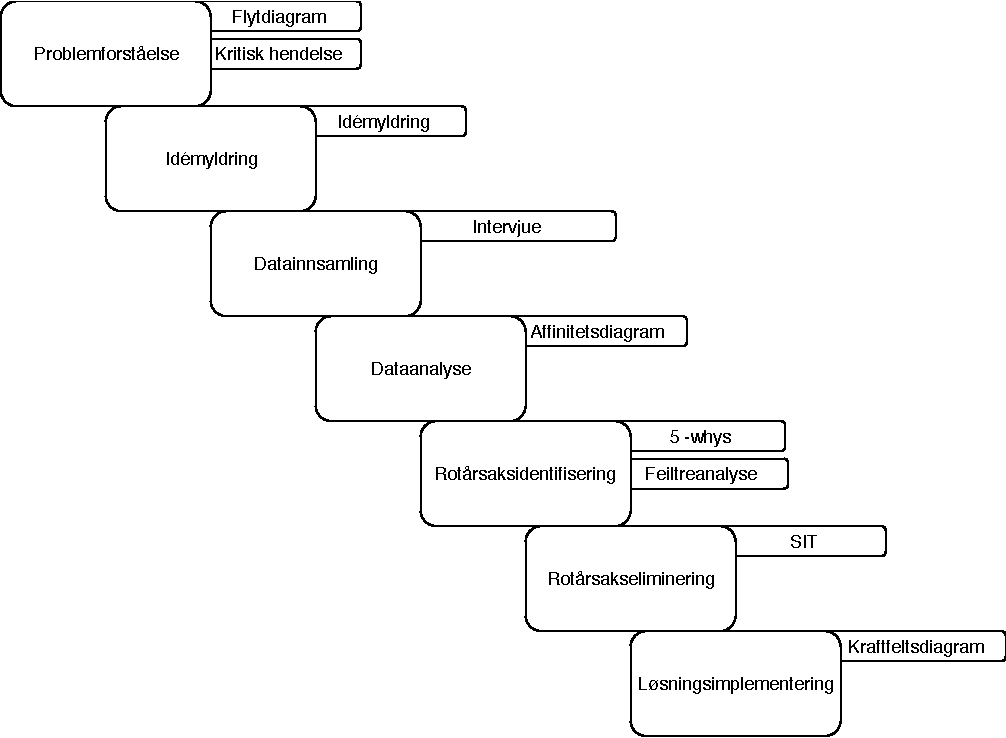
\includegraphics[scale=0.7]{case_3/bilder/Prosess_case_3.pdf}
    \label{fig:prosess}
    \caption[Rotårsaksanalyseprosessen]{Rotårsaksanalyseprosessen definert av Andersen og Fagerli}
\end{figure}